\section*{A Few Words About GPU Architecture}
\begin{figure}[h]
    \centering
    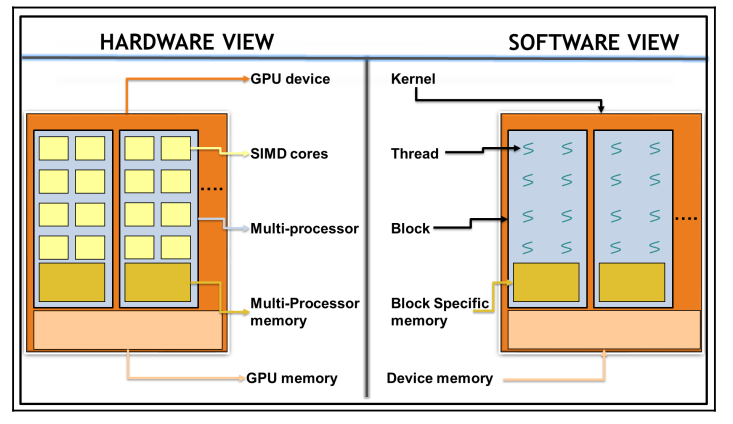
\includegraphics[width=0.8\textwidth]{figures/architecture.png}
    \caption{CUDA Hardware and Programming Model Overview}
    \label{fig:figures-architecture-png}
\end{figure}

Essentially,
\begin{table}[h]
    \centering
    \caption{CUDA Software-Hardware mapping}
    \label{tab:mapping}
    \begin{tabular}{c | c | c}
    \textbf{Software} &  & \textbf{Hardware} \\
    CUDA Thread & executes on/as & CUDA Core/ SIMD Core\\
    CUDA Block & executes on & Streaming Multiprocessor \\
    GRID/kernel & executes on & GPU Device
    \end{tabular}
\end{table}

CUDA threads are more lightweight and provide faster context switches
than CPU threads because of larger register size and hardware-based
scheduler. The thread context is stored in the registers, as opposed
to being on the cache in CPUs.

CUDA blocks execute on a single streaming multiprocessor (SM). All
the threads of a block can only execute on one SM. In general, a GPU
may have multiple SMs. The CUDA programming model allows for
communication between threads in the same block; threads belonging
to different blocks cannot communicate/synchronize.

CUDA provides a \texttt{cudaDeviceProp} data type along with
associated functions that can be used to get the properties of the
device(s) that can communicate with host.

\section*{Error reporting in CUDA}
Errors are managed by the host code. Most CUDA functions return an
enumation type \texttt{cudaError\_t}, with \texttt{cudaSuccess} being
code 0. Here is a typical example.

\begin{minted}{c}
cudaError_t e;
e = cudaMemcpy(...);
if (e)
    fprintf(stderr, "Error: %s\n", cudaGetErrorString(err));
\end{minted}

Kernel launches are always \texttt{void} return-type. So, there is
also a very handy function \texttt{cudaGetLastError()}

\begin{minted}{c}
MyKernel<<<...>>> (...);
cudaDeviceSynchronize();
e = cudaGetLastError();
\end{minted}

Error checking is important in CUDA because the host will continue
executing even if a \texttt{\_\_global\_\_} function (kernel) has
crashed.

